%  Scenario of the system
%
To create a thorough understanding of our system we developed some scenario's in which the product will be used. These scenario's helped us develop state diagrams to understand the internal states of the product so that we could determine protocols to develop an efficient charge-discharge protocol. The actors in the system are the user wearing the wristband, other users that the user can interact with and the system will be portrayed by the energy bar, energy checkpoints and an online server. The latter actors will be discussed more extensive in Section \ref{sec:internet}. The scenario's are portrayed from the perspective of a central user. The perspectives of the energy bar and checkpoint are considerable less complex and follow the perspective of the central user intuitively. 

The use case diagram in figure %\ref{fig:usecase} 
displays the interaction of a user, its friends and other users with the WeLight system. Concerning the wireless power transfer system a user can either charge of get charged by other users and should indicate when it is in need for energy. The product should also still execute its prior tasks which is executing the light show in certain areas where the shows are held, when it is capable to do so in energy terms. These terms will be discussed more in detail in Section \ref{sec:state} and Section \ref{sec:charging}. The internet of things in our system is displayed by the check in mechanism that sends data to a server. The server can then determine some recommendations for the user and his friends and can notify both. This will be discussed more into detail in Section \ref{sec:internet}.
%
%------------------- Use Case image
%\begin{figure}[h!]
%\centering
%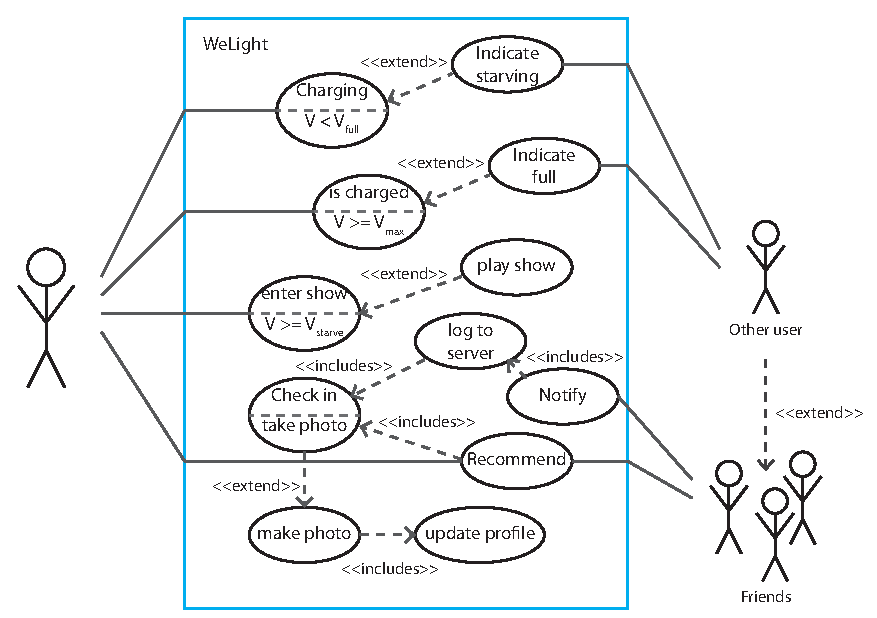
\includegraphics[width=0.8\textwidth]{usecase.pdf}
%\caption{Use case diagram of the WeLight system}
%\label{fig:usecase}
%\end{figure}

The sequence diagrams display the different use cases. Figure %\ref{fig:sequenceshow}
displays regular use of the system in its original design. A show object can detect user IDs by means of RFID tags and then send the instructions via RF signals to the wristbands. These will update their state and loop as long as the battery has a higher energy level than $V_{full}$ as determined in Section \ref{sec:charging}. Figure %\ref{fig:sequencecharge}
follows this sequence and is initiated whenever the energy level of the battery falls below $V_{full}$. It will indicate towards the environment and other users that the battery is starving. The user can then ask another user for energy or visit an energy bar untill $V_{full}$ is exceeded again. When $V_{max}$ is reached the inidication light will turn green as further charging will have no effect.
%
%------------------- Sequence diagram image
%\begin{figure}[h!]
%\centering
%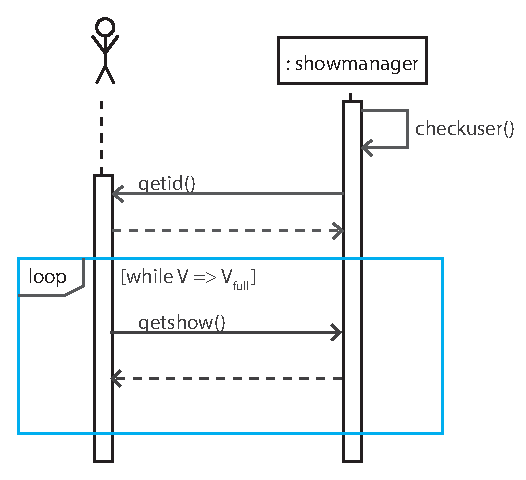
\includegraphics[width=0.8\textwidth]{sequenceshow.pdf}
%\caption{Sequence diagram of regular use of the product}
%\label{fig:sequenceshow}
%\end{figure}

%
%------------------- Sequence diagram image
%\begin{figure}[h!]
%\centering
%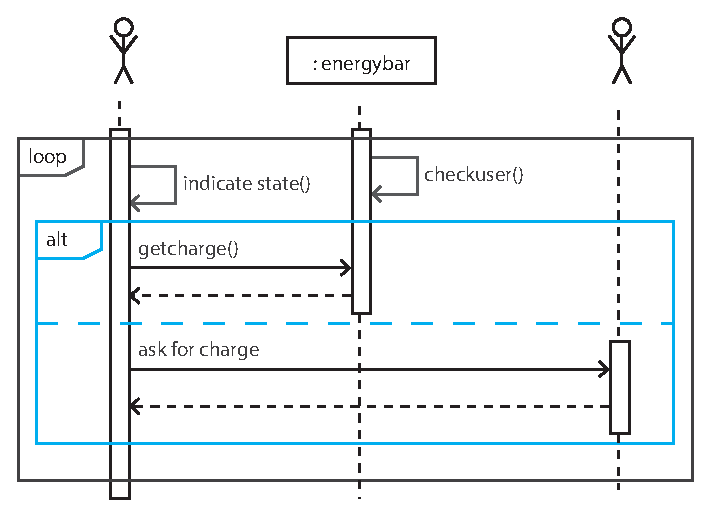
\includegraphics[width=0.8\textwidth]{sequencecharge.pdf}
%\caption{Sequence diagram for charging the system}
%\label{fig:sequencecharge}
%\end{figure}

Figure %\ref{fig:sequenceinternet}
shows the sequence diagram whenever a user connects to a checkpoint at the festival. Information about the time of the log, the position of the checkpoint and thus the concurrent nearest festival podium and the user ID is collected and send to the server. The database compares the information with the users personal profile online and the current festival schedule and returns a recommendation. The user can select to inform his/her friends available on the personal profile. They might even add a personal message in order to agree on a meetingpoint. 

%
%------------------- Sequence diagram image
%\begin{figure}[h!]
%\centering
%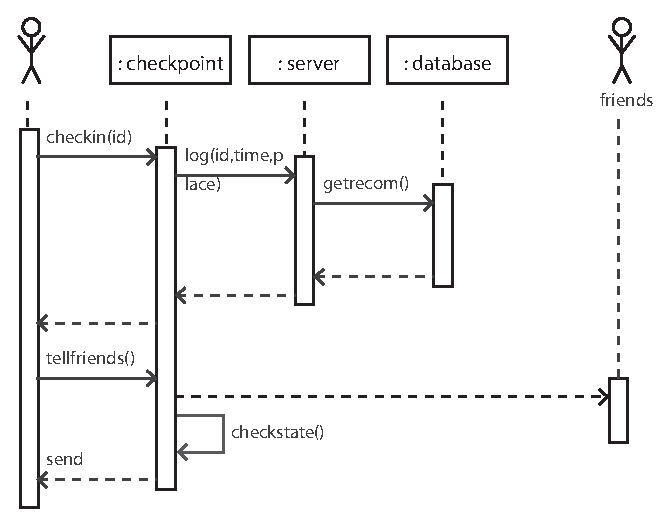
\includegraphics[width=0.8\textwidth]{sequenceinternet.pdf}
%\caption{Sequence diagram of the internet of things}
%\label{fig:sequenceinternet}
%\end{figure}

